\documentclass[12pt, letterpaper]{article}
\usepackage{graphicx} % Required for inserting images
\usepackage{hyperref}
\usepackage{listings}
\usepackage{amssymb}
\usepackage{amsmath}
\usepackage[english]{babel}
\usepackage{nicefrac, xfrac}
\usepackage{mathtools}
\usepackage[table,xcdraw]{xcolor}
\definecolor{light-gray}{gray}{0.95}
\definecolor{sap}{RGB}{130, 36, 51}
\definecolor{lg}{RGB}{102, 161, 95}
\usepackage[paper=a4paper,left=20mm,right=20mm,bottom=25mm,top=25mm]{geometry}
\newcommand{\code}[1]{\colorbox{light-gray}{\texttt{#1}}}
\newcommand{\shelll}[1]{\colorbox{black}{\textcolor{white}{\texttt{#1}}}}
\newcommand{\shell}[1]{\colorbox{black}{\textcolor{white}{\texttt{casufrost@debian:$\sim$\$ #1}}}}
\newcommand{\codee}[1]{\colorbox{white}{\texttt{#1}}}
\newcommand{\acc}{\\\hphantom{}\\}
\newcommand{\dete}{{\rightarrow}}
\newcommand{\fdot}{{\(\bullet\) }}
\newcommand{\boxedMath}[1]{\begin{tabular}{|c|}\hline \texttt{#1} \\ \hline\end{tabular} :}
\title{Progettazione di Algoritmi}
\author{Marco Casu}
\date{\vspace{-5ex}}
\begin{document}



\maketitle
\begin{figure}[h]
    \centering{
    
\includegraphics[width=1\textwidth ]{images/cop.jpg}
    }
\end{figure}
\newpage 
\tableofcontents
\newpage
\section{Grafi}
\subsection{Introduzione e Definizioni}
Un grafo, è una coppia $(V,E)$, dove $V$ è un insieme di \textit{nodi o vertici}, ed $E$ un 
insieme di archi che collegano i nodi. Un grafo è detto \textbf{semplice} se, per ogni 
coppia di nodi, essi sono collegati da al massimo un arco, e non esistono dei cicli su 
un singolo nodo. Nel corso ci occuperemo di \textit{visitare} i grafi in 
profondità ed in ampiezza (concetti che verranno ripresi più in avanti). \acc 
Un grafo, può vedere i suoi archi \textit{orientati}, in questo caso si dice che 
il grafo è \textbf{diretto}. Due nodi sono \textbf{adiacenti} se collegati da un arco, 
ed il \textbf{grado} di un nodo non è altro che il numero di nodi adiacenti ad esso.\begin{center}
    \includegraphics[width=1\textwidth ]{images/defGrafi.eps}
\end{center}
Esiste un problema classico dal 1700, noto come \textit{problema dei ponti di Königsberg}, 
si consideri la seguente città posta nei pressi di un fiume che la divide in diversi settori, collegati 
da appositi ponti, rappresentata con il seguente grafo :\begin{center}
    \includegraphics[width=1\textwidth ]{images/konigsberg.eps}
\end{center}
Ci si chiede se è possibile passeggiare per la città, visitando tutti i settori, senza passare per due volte 
sullo stesso ponte. Consideriamo il modello del grafo, una passeggiata su un grafo non è altro che una 
sequenza ordinata di vertici ed archi che si alternano, come : $v_0,e_1,v_1\dots, e_k,v_k$.
Esiste una passeggiata su questo grafo, ossia una sequenza che non vede ripetizioni degli archi?\acc 
\textbf{Osservazione} : Per visitare un nodo è necessario passare per due archi, uno entrante ed uno uscente. 
Se entriamo in un nodo di grado 3, resterà un arco non visitato, per visitarlo sarà necessario entravi nuovamente 
da tale arco, per poi uscire da un altro precedentemente già visitato (questo ovviamente se non si comincia la 
passeggiata dal nodo in questione).\acc 
Ci rende chiaro il seguente fatto : Se il grado di un nodo $x$ è dispari, a meno che la passeggiata non inizi 
o finisca su $x$, uno dei suoi archi verrà attraversato più di una volta. \textit{Eulero} studiò questo problema, 
si dice infatti che la passeggiata su un grafo è \textbf{euleriana} se non si passa 2 volte sulle stesso arco.\acc 
Si consideri però il seguente grafo :\begin{center}
    \includegraphics[width=1\textwidth ]{images/nonConnesso.eps}
\end{center}
Un grafo si dice \textbf{connesso} se, per ogni coppia di vertici, essi sono collegati da una passeggiata, 
ossia è possibile raggiungere un vertice partendo da un altro. Le precedenti osservazioni ci portano al 
seguente risultato.\acc 
\textbf{Teorema (Eulero)} : Un grafo ha una passeggiata euleriana se e solo se è connesso, ed 
esistono al massimo 2 vertici di grado dispari.\acc 
Il fatto che sono concessi 2 vertici di grado dispari, è dato dal fatto che essi saranno l'inizio e la fine 
della passeggiata.
\subsection{Rappresentazione Fisica}
Che struttura dati possiamo utilizzare per rappresentare un grafo? Vediamo due alternative : \begin{itemize}
    \item \textbf{Matrice di Adiacenza} - Utilizziamo una matrice $n\times n$, dove \(n\) è il numero di 
    nodi del grafo. Nella posizione \(i,j\) ci sarà 1 se il vertice \(v_i\) è adiacente al vertice 
    \(v_j\), altrimenti 0. Il costo di "\textit{check}" per l'adiacenza di due vertici è costante, basta 
    consultare un entrata della matrice, nonostante ciò, lo spazio che occupa tale rappresentazione è 
    \(O(n^2)\).
    \item \textbf{Liste di Adiacenza} - Ad ogni vertice del grafo è associata una lista, contenente tutti 
    i suoi vertici adiacenti, per controllare se due vertici sono adiacenti, è necessario fare una ricerca 
    lineare su tale lista, ed ha costo $\displaystyle O(deg(v))$, dove \(v\) è il vertice sulla 
    quale si sta effettuando la ricerca, ed è ovviamente limitato da \(n-1\) (numero di vertici).\acc
    Le dimensioni della struttura dati sono $\displaystyle O\big(n + \sum_{v\in V(G)}deg(v)\big)$.
\end{itemize}
Nel caso in cui un grafo dovesse vedere ogni vertice adiacente a tutti gli altri, la ricerca costerebbe 
\(O(n)\) e le dimensioni sarebbero \(O(n^2)\), ciò differisce però dal caso reale, la rappresentazione con 
liste di adiacenza risulta un buon compromesso fra costo computazionale e dimensioni.
Sarà usuale denotare \(m\) il numero di archi e \(n\) il numero di vertici.
Le liste di adiacenza occupano quindi spazio $O(n+m)$,  si osservi inoltre la 
seguente identià : $$\sum_{v\in V(G)}deg(v)=2\cdot m\text{ dove }m:=|E|$$
\subsection{Ricerca di un Ciclo}
\textbf{Definizione} : Un \textit{ciclo} in un grafo, non p altro che un \textit{sottografo connesso} dove 
ogni vertice è di grado 2. Identifica un "cammino circolare", e la ricerca dei cicli nei grafi è un 
problema molto noto.\begin{center}
    \includegraphics[width=0.8\textwidth ]{images/ciclo.eps}
\end{center}
Consideriamo adesso un problema, vogliamo definire un algoritmo che, dato in input un grafo \(G=(V,E)\), dove ogni 
vertice ha grado maggiore o uguale a 2, restituisca in output un qualsiasi ciclo presente nel grafo, mantenendo 
un costo computazionele $O(n+m)=O(|V|+|E)$. 
\begin{quote}
    Si consideri la seguente \textit{idea} informale di soluzione : \end{quote}  
    Ogni vertice ha almeno 2 nodi adiacenti, è quindi sempre possibile entrare in un vertice ed uscirne da un
    arco diverso da quello dalla quale si è entrati. Si parte da un qualsiasi vertice nel grafo, e si procede 
    selezionando uno qualsiasi dei due nodi adiacenti successivi, almeno uno dei due non sarà quello dalla 
    quale si è entrati, procederemo in questa maniera camminando in maniera casuale sul grafo, finchè non troveremo 
    un nodo che è stato già visitato in precedenza, ciò indica che si è eseguito un cammino ciclico.\acc 
Utilizzeremo un vettore con lo scopo di salvare i nodi visitati, il ciclo sarà rappresentato 
dai nodi presenti nel vettore, partendo dall'ultimo elemento, continuando a ritroso fino a trovare il nodo 
identico all'ultimo. Si consideri il seguente esempio in cui gli archi sono contrassegnati dall'iterazione 
dell'algoritmo nella quale sono stati attraversati : 
\begin{center}
    \includegraphics[width=0.8\textwidth ]{images/algoCiclo.eps}
\end{center}
Una volta completato la ricerca del ciclo, elimineremo dal vettore tutti gli elementi a partire dal primo 
fino all'elemento antecedente a quello identico all'elemento finale. \begin{center}
    Pseudocodice 
\end{center}
\code{Input} : Un grafo $G=(V,E)$.\\
\code{Output} : I nodi di un sottografo di \(G\) che è un ciclo.\\\hphantom{}\\
\hphantom{ident}\codee{x = V[random]}\color{lg}\textit{// Un vertice a caso}\color{black}\\
\hphantom{ident}\codee{W=[x]}\color{lg}\textit{// Inizializzo il vettore output}\color{black}\\
\hphantom{ident}\codee{current = V}\\
\hphantom{ident}\codee{y=adiacente di x}\color{lg}\textit{// Un adiacente a caso}\color{black}\\
\hphantom{ident}\codee{next=y}\\
\hphantom{ident}\codee{while(next$\notin$ W)\{}\\
\hphantom{ident}\hphantom{ident}\codee{W.append(next)}\\
\hphantom{ident}\hphantom{ident}\codee{current=next}\\
\hphantom{ident}\hphantom{ident}\codee{if ($1^\circ$ adiacente di current$\ne$W[W.lenght-2])\{}
\color{lg}\textit{// Il penultimo}\color{black}\\
\hphantom{ident}\hphantom{ident}\hphantom{ident}\codee{next = $1^\circ$ adiacente di current}\\
\hphantom{ident}\hphantom{ident}\codee{\}else\{next = $2^\circ$ adiacente di current}\\
\hphantom{ident}\codee{\}}\\
\hphantom{ident}\codee{while(W[0]$\ne$next)\{}\\
\hphantom{ident}\hphantom{ident}\codee{W.remove(W[0])}\color{lg}\textit{// Rimuove il primo elemento}\color{black}\\
\hphantom{ident}\codee{\}}\\
\hphantom{ident}\codee{return W}\acc 
Qual'è la complessita di tale algoritmo? Entrambi i cicli \code{while} eseguono \(O(n)\) iterazioni, il 
fatto è che, nel primo ciclo while, il controllo \code{next$\notin$W} deve scorrere comunque tutto il vettore, 
rendendo il costo dell'algoritmo \(O(n^2)\), non rispettando le specifiche iniziali, ossia \(O(n+m)\).
\end{document}
